\chapter{Assessing Scalability}

\section{Scalability: Quantitative Methodology}

\begin{figure}
\centering
	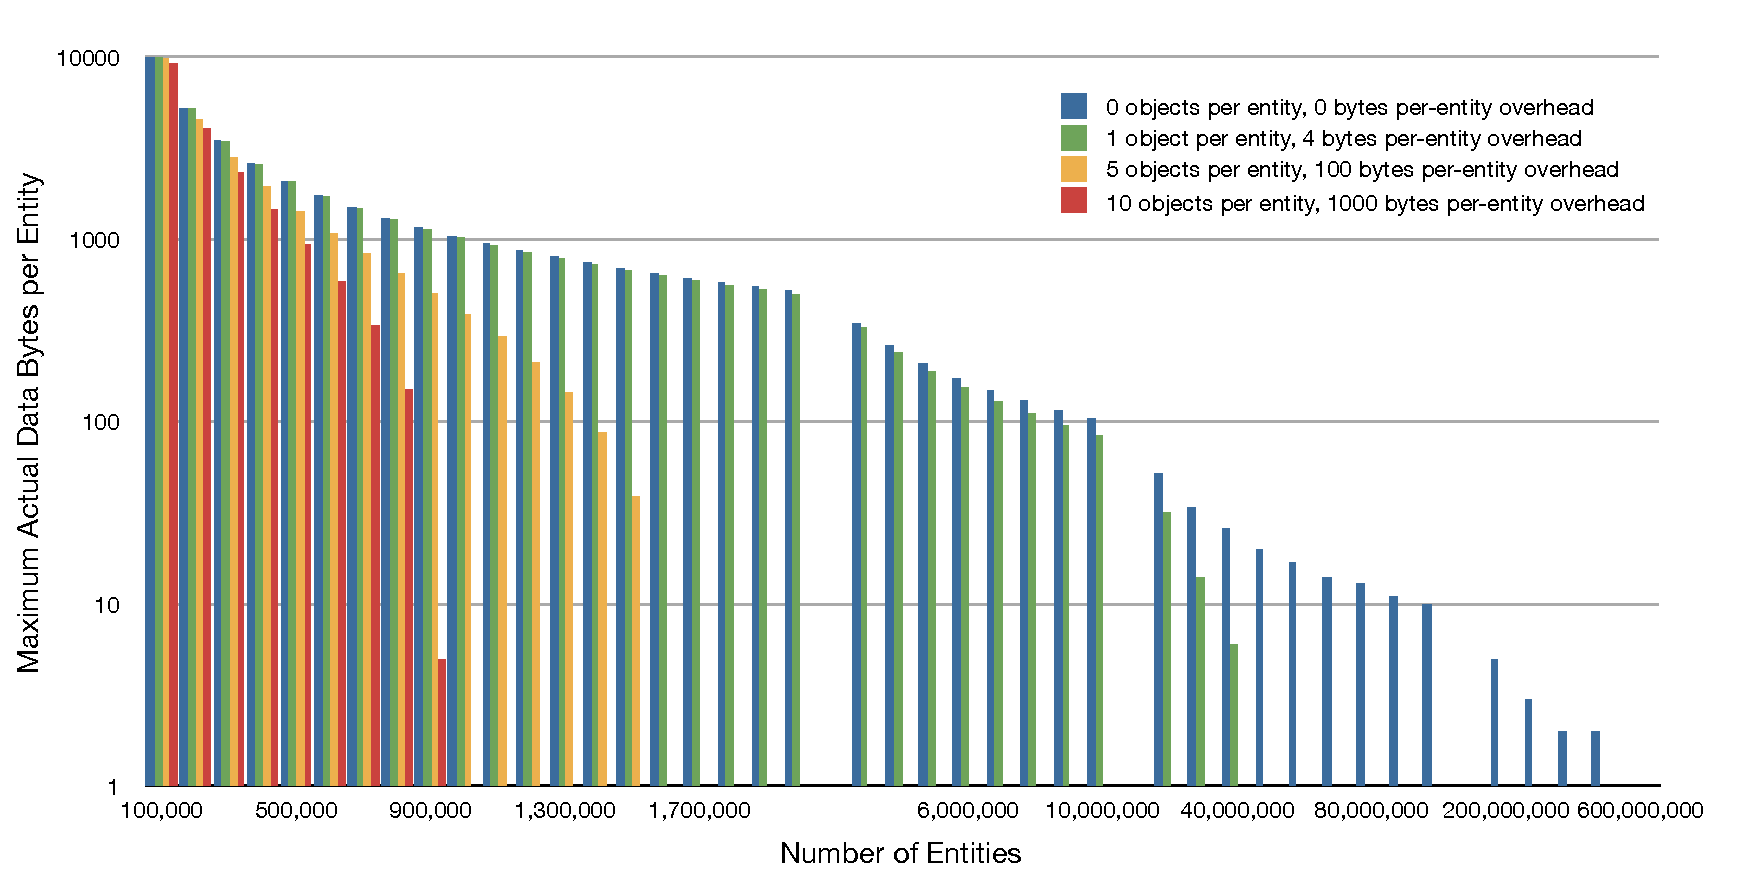
\includegraphics[width=\textwidth]{part3/Figures/assessing/maxActualData}
	\caption{The amount of actual data you can store in your entities depends on
	the degree of delegation in your entities, and the per-entry overhead of the collection in which these entities
	reside. This chart assumes a limit of 1 gigabyte of Java heap.}
	\label{fig:maxActualData}
\end{figure}

TODO: write this section, explaining \autoref{fig:maxActualData}, or delete it.

\section{Example: Representing a Graph}

When representing relationships between entities, using standard object oriented
practices, you are severely limited in the number of entities and relationships
that you can store. Doing so in a straightforward manner, one that obeys object
oriented practices, is very similar to the task of representing a graph of nodes
and edges. For example, when caching data from a relational database in the Java
heap, the entities (rows in a database table) and relations (columns that contain
indices into tables) become the nodes and edges in a graph.

%\begin{example}{Storing a Graph}
If a graph has a great many nodes and edges, you must design its storage
carefully. Consider the small example illustrated in 
\autoref{fig:exampleGraph}. There are several ways to implement the abstract
data types, of nodes and edges, shown in that figure. Each strategy has its
positives and negatives, depending on whether ease of maintenance or memory
consumption are of primary importance.
%\end{example}

\begin{figure}
\centering
\subfigure[Example graph.]{
\label{fig:example-storing-relations-graph}
\shortstack{
	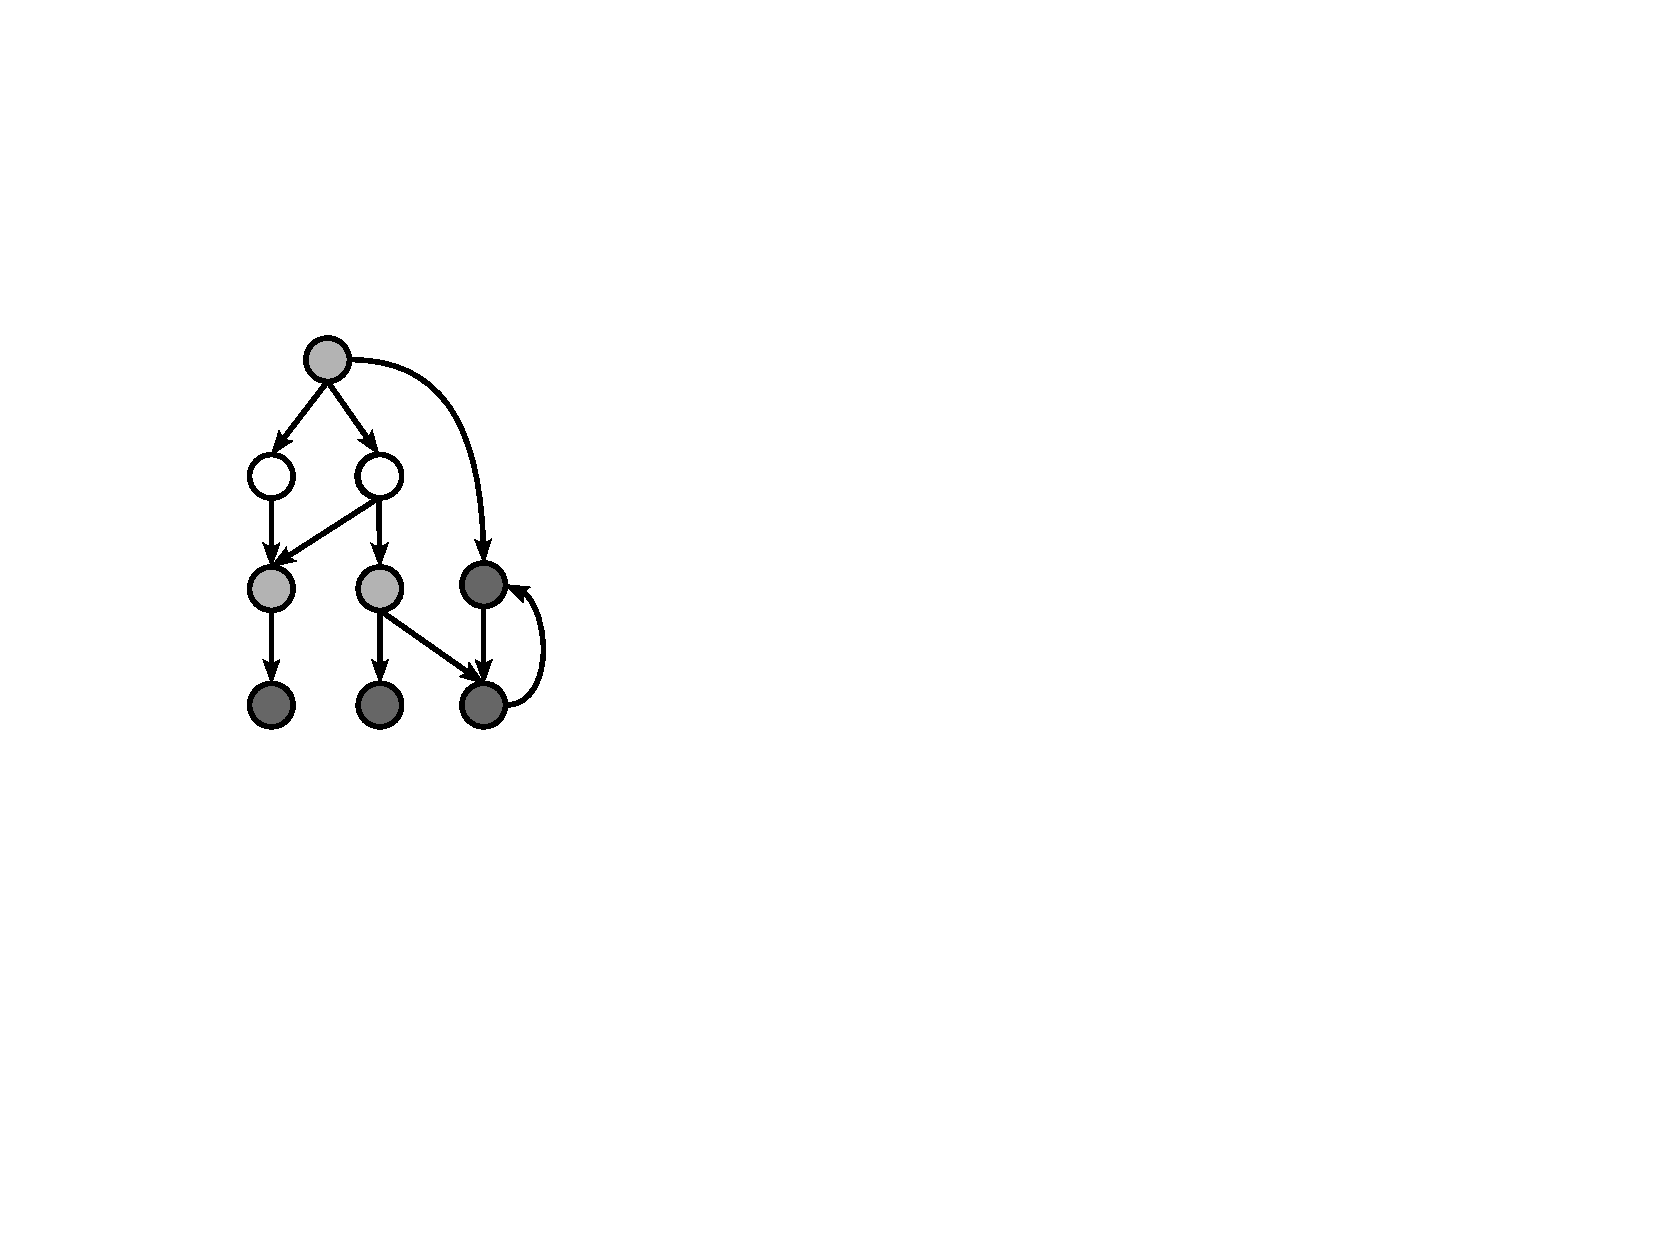
\includegraphics[width=0.3\textwidth]{part3/Figures/assessing/exampleGraph}
	\\ \vspace{5mm}
	}
}
\qquad
\begin{subfloat}
\label{fig:graph-interfaces}
\begin{minipage}[b]{0.45\textwidth}
\begin{figurelisting}
interface Graph {
	Set<Node> getNodes();
	Set<Edge> getEdges();
}
interface Node {
	Color getColor();
	Set<Edge> getChildren();
	Set<Edge> getParents();
}
interface Edge {
	Node getFrom();
	Node getTo();
}
enum Color {
	White, LightGray, DarkGray
}
\end{figurelisting}
\end{minipage}
\caption{Abstract data types for nodes and edges.}
\end{subfloat}
	\caption{An example generic graph of three colors of nodes.}
	\label{fig:exampleGraph}
\end{figure}

\begin{figure}
\centering
\begin{subfloat}
\begin{minipage}[b]{0.3\textwidth}
\begin{figurelisting}
class Node {
   Color color;
   Set<Edge> parent;
   Set<Edge> child1;
   Set<Edge> child2;
}
\end{figurelisting}
\end{minipage}
\caption{Concrete classes}
\end{subfloat}
\quad
\begin{subfloat}
\begin{minipage}[b]{0.5\textwidth}
\begin{figurelisting}
public Node(Color color) {
   color = color;
   parents = new HashSet<Edge>();
   children = new HashSet<Edge>();
}
\end{figurelisting}
\end{minipage}
\caption{Node constructor that uses the default \class{HashSet} constructor.}
\label{fig:node-obvious-constructor}
\end{subfloat}
\caption{A straightforward implementation of the Node interface.}
\label{fig:node-obvious-impl}
\end{figure}

\autoref{fig:graph-interfaces} shows the interfaces for a \class{Graph},
\class{Node}, and \class{Edge} that one must implement. A common implementation
strategy, applied to the \class{Node} and \class{Edge} data types, is a
straightforward mapping of interfaces to concrete classes.
\autoref{fig:node-obvious-impl} shows such an implementation for the
\class{Node} data type. Following this
strategy, the \class{Node} class has three fields, to store its \class{Color}
and the relations to children and parents; these relations are implemented with a
standard collection, likely a \class{HashSet}. The \class{Edge} class has two
fields, to store pointers to the source and target nodes. This implementation is
easy to implement. It is also easy to maintain: changes to the interfaces can be
directly mapped to changes to the implementation, because the two are parallel
versions of each other. The nodes and edges, and relations between them, are
objects that can be manipulated using normal object oriented practices; e.g. you
can write \texttt{node.getChildren().get(5).getTo()\-.getColor()}, which reads
as a fairly natural, albeit verbose, expression of what you intend.

\paragraph{A Straightforward Implementation}
Without any thought for memory concerns, the constructor for a node would be as
shown in \autoref{fig:node-obvious-constructor}. In this implementation, the
memory cost per node is three pointers plus two collections of default size. As
\autoref{tab:collection-costs} shows, the the default constructor of a
\class{HashSet} allocates an array to hold 16 elements; the per-collection cost
is 136 bytes and the per-entry cost is 28 bytes. If, on average, a node has one
parent and 2 children, then each node will consume one object header plus $3*4
+2*136 + 2*3*28$, or $464$ bytes; using \class{ArrayList} instead of a hash map
would cost $3*4+ 2*(80 + 10*4)$, or $264$ bytes. Both choices result in 24\% of
memory wasted on null pointers.
% hashset: 112=14 entries at 4 bytes each, times two for parents and children 
% arraylist: 68=8 entries at 4 bytes each, times two for parents and children
The 136 bytes (29\%) spent on the parent collection is unnecessary, for those
nodes that have exactly one parent. Even an optimally structured set which
includes just one pointer for a set with one entry would still impose two pointer
costs to reference a single parent node: one pointer to reference the set, one
for the set to reference the parent node.

In addition to the cost of the nodes are the cost of the edges objects. By
objectifying each edge, this implementation pays a cost of one object header
plus two pointers, or 24 bytes (20 bytes, before rounding up to an 8-byte
alignment boundary). For the example with an average of one parent and two
children per node, the effective cost per node is $264 + 3*24$, or $336$ bytes.

Ideally, a node with one parent and two children should consume four pointers, or
16 bytes: one to reference a \class{Color}, one to reference the parent node, and
two pointers to reference the children. The disparity between this optimal value
and the cost of the standard implementation is 320 bytes. A inspection of
\autoref{fig:maxActualData} shows that this implementation, with 16 bytes of
actual data and 320 bytes of overhead, can support at most 2.7 million nodes per
gigabyte of heap. An ideal implementation, with no storage costs beyond the
necessary 16 bytes of pointers, would be able to support at most 65 million nodes
per gigabyte of heap.

\paragraph{Optimizing the Implementation}
By specializing your code to handle only a limited degree of functionality, you
can achieve a fair degree of compactness without much effort. If every node has
exactly the same number of incoming and outgoing edges, an easy alternative
implementation presents itself. You can specialize the implementation for this
structural special case, and thereby eliminate the waste that comes from allowing
a flexible number of incident edges.
\autoref{fig:node-tuned-impls}a shows an implementation of the \class{Node}
interface that does away with collections. On top of the ideal implementation,
the cost per node is one object header plus two pointers for each of the three
\class{Edge} objects. On top of the 16 byte ideal cost, this implementation costs
an additional $3*(2*12 + 2*4)$ bytes, for a total of 112 bytes. This cost is one
third that of the initial implementation, though 7 times the cost of the ideal
implementation. This implementation supports just over 9 million nodes per
gigabyte of heap.

Even if many nodes have no parents, or fewer than two children, this specialized
implementation remains preferable to the original one that uses collections. This
is because an empty collection consumes no less than then the one pointer that
this collection-free implementation costs; this is the case if you point to the
singleton \code{Collections.emptySet()}. In the case when a node has one child,
then a set must be allocated, whose expense, even if the set has only a single
entry, will always be higher than a single pointer.

\begin{figure}
\centering
\begin{subfloat}
\begin{minipage}[b]{0.38\textwidth}
\begin{shortlisting}
class Node {
   Color color;
   Edge parent;
   Edge child1;
   Edge child2;
}
\end{shortlisting}
\end{minipage}
\label{fig:node-no-collections}
\caption{No collections}
\end{subfloat}
\qquad
\begin{subfloat}
\begin{minipage}[b]{0.38\textwidth}
\begin{shortlisting}
class Node {
   Color color;
   Node parent;
   Node child1;
   Node child2;
}
\end{shortlisting} 
\end{minipage}
\caption{No objectified Edges}
\label{fig:node-no-Edge-objects}
\end{subfloat}
\caption{Two implementations that have been specialized for the case where
no object has more than one parent and no more than two children.}
\label{fig:node-tuned-impls}
\end{figure} 

\autoref{fig:node-tuned-impls}b shows a yet more highly optimized \class{Node}
implementation that stores pointers to \class{Node}s, rather than \class{Edge}s.
One somewhat extreme variant of this implementation does not store \class{Edge}
objects at all. This \class{Edge}-free implementation approaches the ideal
implementation, in its capacity for storing large graphs. You must still pay one
object header per node, for the \class{Node} objects themselves. Thus, this
impementation has a per-node memory cost of 16 bytes for the pointers plus 12
bytes for the header. At this unit cost, a one gigabyte heap would support at
most 38 million nodes.

Though quite scalable, this implementation presents several complications. First
is the obvious limitation to at most one parent and at most two children per
node. Second, an \class{Edge}-free storage strategy dictates that the
\class{Node} API also be updated so that \code{Node.getChildren()} and
\code{getParents()} return a set of nodes, rather than a set of edges. You
cannot avoid storing \class{Edge} objects and yet support an external interface
of \class{Edge}s The same issue holds for an implementation that stores only a
single parent pointer: how can one efficiently support an interface that expects
a set of edges, if the storage contains only a single pointer? If you don't make
this API change, and instead choose to return facades that route the edge
operations properly, users of the API will be in for some surprises. The
following implementation does not work:
\begin{shortlisting}
public Set<Edge> getParent() {
   Set<Edge> set = new HashSet<Edge>();
   set.add(parent);
   return set;
}
\end{shortlisting}
This implementation will not reflect any updates that the caller makes to the
returned set. It also violates the implicit reference-equality contract of
interfaces in Java: two calls to the \code{getParents()} interface must have
reference, i.e. \code{==}, equality. If possible, you can update
the written specification for the interface to indicate that a read-only
\emph{copy} of the parent set is returned. Unforunately, neither of these
policies can be statically enforced, and are hence prone to misuse.
Worse, if the interface design is out of the
scope of changes you can make, then you are out of luck and must cache the
returned set somewhere, so as to preserve reference equality.

Third, in addition to being quite expensive, in creating a set for every call to
\code{getParent}, this implementation lacks in expressive power compared to the
other implementations presented so far. For example you will find it more
difficult to extend the graph interface to support edge labels. Adding edge
labels with low overhead is not impossible, but requires some careful planning,
and thinking outside the Java box.

\paragraph{Difficulties of Supporting Edge Properties in Optimized
Implementations} If the API method \code{Node.getChildren()} returns a set of
nodes, rather than a set of edges, then the code to access an edge label of the
second child of a node can no longer be
\texttt{node.getChildren().\-get(1).getLabel()}. This way of traversing the graph
leads to a node, not an edge! Instead, edge labels must be fetched from some
larger entity, such as the graph model itself: e.g. \texttt{graph.getEdge(from,
to).getLabel()}, or \texttt{graph.getEdgeLabel(from, to)}. Without some care,
every edge label query will require a hash table lookup. Your design necessitates
storing the edge labels in a side data structure, one whose elements are not
directly connected, via pointers, to the nodes.

Storing edge labels in a parallel map-like structure makes sense only if a small
fraction of the edges have labels. Otherwise, the costs of the map infrastructure
may very well overwhelm the cost of the labels. Let's say that each label
consumes 4 bytes of actual data. A quick look at
\autoref{tab:collection-costs} shows that the per-entry cost of a \class{HashMap}
is 28 bytes. If, without edge labels, your implementation supports 38 million
nodes per gigabyte of heap (recall that this implementation supports at most
one parent and two children per node)
% 38 million is 16 bytes of data plus 12 bytes of header per node
then adding edge labels, in an ideal fashion that adds no additional overhead,
will decrease your capacity to 26.8 million nodes per gigabyte --- a reduction
in capacity of 30\%.
% 33.5 million is 16 + 12 + 4 bytes per node
If you store them in a \class{HashMap}, your capacity will decrease to at most
10.3 million nodes per gigabyte: the map costs 28 bytes per entry,
plus you need to create some sort of \class{Pair} object to house the source and
target nodes that form the map's key, plus you need to create a wrapper object to
house the edge label itself.
% 16 of actual data plus 12 bytes of header for the node 12+4+4 for the edges 4
% of actual data for the edge label 28 for the $Entry 12+4 for the Value 12+4+4
% for the Key
In contrast to the 30\% reduction of an ideal implementation of edge labels,
this straightforward implementation results in a 73\% reduction in capacity. In
this case the penalty of using a map is especially high because the starting
implementation, i.e. one supporting 38 million nodes per gigabyte, was fairly
highly tuned. The more highly tuned your memory design, the larger the negative
repercussions of subsequent bad choices. For example, if your starting
implementation supported 22 million nodes per gigabyte, then the penalty of a
map-based implementation of edge labels would be a somewhat lower 61\%.

A more efficient approach, if you have the luxury of modifying the \class{Node}
implementation directly, or subclassing it and overriding factory methods, is to
inline the edge labels directly into the \class{Node} class:
\begin{shortlisting}
class Node {
   Color color;
   Node parent;
   Node child1;
   Node child2;
   Label parentLabel;
   Label child1Label;
   Label child2Label;
}
\end{shortlisting} 
To avoid any need to maps, though, would require you to update the API for
fetching edge labels. Calling \code{graph.getEdge(from, to).getLabel()} with
this implementation would require an intervening map structure. In contrast,
an API that had the form \code{node.getParentLabel(0)} and
\code{node.getChildLabel(1)} would allow for direct access to the labels,
without a map. Inlining the storage for labels requires a concomitant inlining
of the APIs. Therefore, while this implementation
approaches the optimal capacity, it is not especially desirable, from an
engineering perspective.
 
%\paragraph{Insufficiencies of Pure Object Orientation}
This activity of tuning the original graph implementation has lead to two
difficult ends. First, it is difficul to support nodes with widely
varying numbers of parents and children. If all nodes had only a very small number of incident
edges, or a very large number, then specialized implementations are possible.
Second, optimizing storage has come at the expense of easy extensibility; one
can remove the use of \class{Edge} objects, but, to support edge labels 
requires either expensive maps to parallel data structures, or 
pollution of data types not directly connected to the planned extension.

\subsection{Supporting Singleton Sets}
\index{Singleton Collections}

% If the distribution of the sizes of these sets is starkly bimodal, where most
% of the sets are either fairly large, or

One common case, when using collections, is that many of them contain zero or
only a single element. It seems silly to pay the expense of a full-fledged
collection for these special cases. The Java standard library offers has a
partial solution to the case of many empty collections, in the form of the family
of factor methods that include \code{Collections.emptySet()} and
\code{Collections.emptyList()}.
\index{Empty Collections}
These are partial solutions, because they only handle the case of unchanging
collections. There is no provision, in the standard libraries, for optimized
storage of single-entry collections. Consider our graph from the previous
section:
\begin{shortlisting}
class Node {
	Color color;
	Set<Edge> parents;
	Set<Edge> children;
}
\end{shortlisting}
The previous section proposed an optimization for the special case of nodes with
at most one parent. If this were always the case, for every single node ever
created by your application, then it is valid, and indeed a good idea,
to change the \class{Node} class definition to inline the pointer to that
potential part. If it is only sometimes the case, then this trick does not work.

You can regain a degree of flexibility, at the expense of some added coding
complexity. First, you must update the \class{Edge} interface to indicate that an
edge is also capable of acting as a singleton set of edges:
\begin{shortlisting}
interface Edge extends Set<Edge> {
}
\end{shortlisting}

Second, you must update your edge implementations to implement the boilerplate of
the \class{Set<Edge>} interface; this part is straightforward. For example,
you must implement all of the mutating methods, such as insertion and removal,
to thow an unsupported operation exception. This ugliness wouldn't be necessary
if the standard library had an interface that represented an unmodifiable set;
instead, an unmodifiable set is only a hidden implementation constructed via
the \class{Collections.unmodifiable} family of factory methods.

Now you have an edge that is also a singleton set of edges. It then becomes
possible to have a single node implementation that supports arbitrary numbers of
parents, but is also optimized the special case of nodes with only a single
parent. This is possible, without your having to change the fields of the
\class{Node} class in any way: a field \class{Set<Edge> parents} can,
transparently, be either an optimized singleton, or a more general set.

So far, the changes necessary to implement this optimization have been local in
scope. They have not violated any principles of abstraction, because changes have
been isolated to the \class{Edge} details. The final change you need to make
requires some abstraction-violating changes. This implementation of the
constructor and \class{addParent} does not specialize for small collections:

\begin{shortlisting}
class Node {
  public Node() { // constructor
     this.parents = new HashSet<Edge>();
  }
  public void addParent(Node parent) {
     parents.add(new Edge(this. parent));
  }
}
\end{shortlisting} 

In order to take advantage of the edge-as-singleton-set optimization, you must
pollute the node's \code{addParent} implemnetation. Here is an implementation
that optimizes both for empty and singleton sets:

\begin{shortlisting}
class Node {
  public Node() { // constructor
     this.parents = Collections.emptySet();
  }
  public void addParent(Node parent) {
     if (parents.size() == 0) parents = new HashSet<Edge>();
     else if (parents.size() == 1) {
        Edge firstParent = parents.iterator().next();
        parents = new HashSet<Edge>();
        parents.add(firstParent);
     }
     parents.add(new Edge(this. parent));
  }
}
\end{shortlisting} 

This data abstraction violation is unfortunate and only avoidable by
reintroducing the very wrappers you have sought to eliminate. It would be nice if
\code{Edge.add()}, i.e. the implementation of the \class{Set} interface, could
reroute of all pointers to this edge to point to a proper set. However, in Java,
it is not possible to have \code{Edge.add()} change this edge's reference
identity. Doing so would require a level of indirection, where edges are
referenced via \emph{handles}, pointers to pointers, rather than direct
pointers.\index{Handles} An \class{ArrayList} does this, by wrapping an object
around the underlying array. This storage structure offers a degree of
transparency, where the array can be reallocated, or conceivably changed to an
entirely different storage structure without any global changes. The Smalltalk
language\index{Smalltalk} provides a \code{become}
primitive\index{\texttt{become} primitive} that allows for pointer rerouting,
without the use of handles, though at a nontrivial runtime expense. In the worst,
but common, case, every call to \code{become} requires a full garbage collection.

\paragraph{Insufficiencies of Pure Object Orientation}
Using a fully object-oriented Java design, it is impossible to achieve both
compactness of storage and the generality to handle a variety of graph
structures. To do so requires coding in a style that is not conventionally object
oriented.
% what?
%By specifying that the parents of a node are a \class{List<Edge>},
%you are forced to 

